\tikzset{
  declare function={
    normpdf(\x,\mu,\sigma)=1/(\sigma * sqrt(2 * pi)) * exp(-((\x - \mu)^2)/(2 * \sigma^2));
    lognormpdf(\x,\mu,\sigma)=1/(\x*\sigma*sqrt(2*pi))*exp(-((ln(\x)-\mu)^2)/(2*\sigma^2));
  }
}
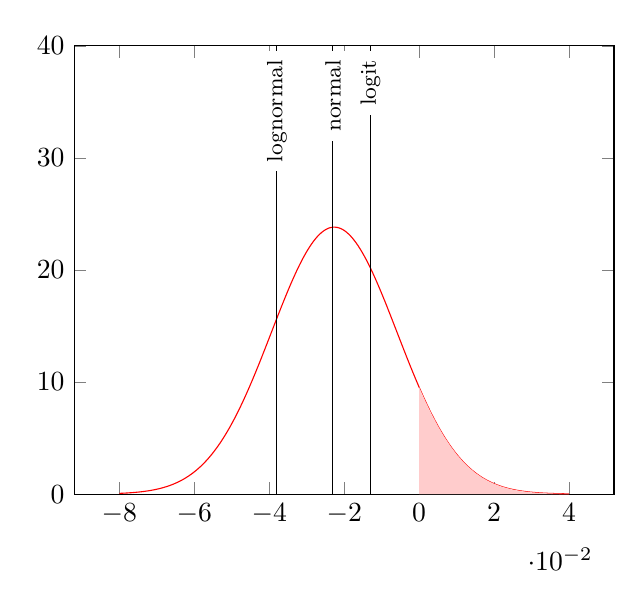
\begin{tikzpicture}
  \begin{axis}[ymin=0, ymax=40]
    \addplot[
      red, 
      domain=-0.08:0.04, 
      samples=201, 
    ] {
      normpdf(x, -2.2657162e-002, 1.6749028e-002)
    };
    \addplot[fill=red!20, draw=none, domain=0:0.04] {
      normpdf(x, -2.2657162e-002, 1.6749028e-002)
    } \closedcycle;
    \addplot[
      blue, 
      domain=-0.08:-0.0001, 
      samples=201, 
    ] {
      -lognormpdf(x, -4.0326920, 1.2417319)
    };
    \tikzstyle{my node}=[
      pos=.99, anchor=east, rotate=90, font=\footnotesize, fill=white
    ]
    \draw[-](-0.013, 0) -- node[my node]{logit} (-0.013, 40);
    \draw[-](-0.023, 0) -- node[my node]{normal} (-0.023, 40);
    \draw[-](-0.038, 0) -- node[my node]{lognormal} (-0.038, 40);
  \end{axis}
\end{tikzpicture}
